% Created by tikzDevice version 0.12 on 2019-02-27 16:26:00
% !TEX encoding = UTF-8 Unicode
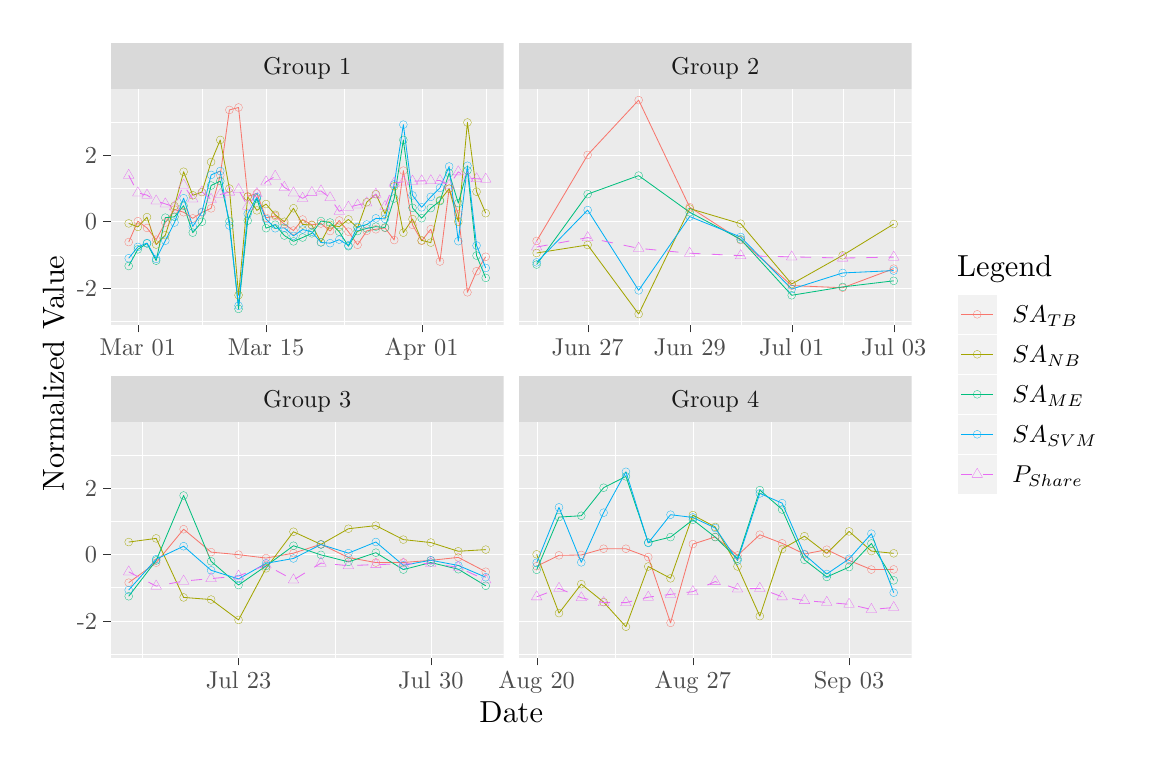
\begin{tikzpicture}[x=1pt,y=1pt]
\definecolor{fillColor}{RGB}{255,255,255}
\path[use as bounding box,fill=fillColor,fill opacity=0.00] (0,0) rectangle (397.48,258.37);
\begin{scope}
\path[clip] (  0.00,  0.00) rectangle (397.48,258.37);
\definecolor{drawColor}{RGB}{255,255,255}
\definecolor{fillColor}{RGB}{255,255,255}

\path[draw=drawColor,line width= 0.1pt,line join=round,line cap=round,fill=fillColor] (  0.00, -0.00) rectangle (397.48,258.37);
\end{scope}
\begin{scope}
\path[clip] ( 30.06,151.03) rectangle (171.97,236.06);
\definecolor{fillColor}{gray}{0.92}

\path[fill=fillColor] ( 30.06,151.03) rectangle (171.97,236.06);
\definecolor{drawColor}{RGB}{255,255,255}

\path[draw=drawColor,line width= 0.1pt,line join=round] ( 30.06,152.41) --
	(171.97,152.41);

\path[draw=drawColor,line width= 0.1pt,line join=round] ( 30.06,176.34) --
	(171.97,176.34);

\path[draw=drawColor,line width= 0.1pt,line join=round] ( 30.06,200.26) --
	(171.97,200.26);

\path[draw=drawColor,line width= 0.1pt,line join=round] ( 30.06,224.19) --
	(171.97,224.19);

\path[draw=drawColor,line width= 0.1pt,line join=round] ( 62.97,151.03) --
	( 62.97,236.06);

\path[draw=drawColor,line width= 0.1pt,line join=round] (114.25,151.03) --
	(114.25,236.06);

\path[draw=drawColor,line width= 0.1pt,line join=round] (165.52,151.03) --
	(165.52,236.06);

\path[draw=drawColor,line width= 0.1pt,line join=round] ( 30.06,164.38) --
	(171.97,164.38);

\path[draw=drawColor,line width= 0.1pt,line join=round] ( 30.06,188.30) --
	(171.97,188.30);

\path[draw=drawColor,line width= 0.1pt,line join=round] ( 30.06,212.23) --
	(171.97,212.23);

\path[draw=drawColor,line width= 0.1pt,line join=round] ( 39.81,151.03) --
	( 39.81,236.06);

\path[draw=drawColor,line width= 0.1pt,line join=round] ( 86.13,151.03) --
	( 86.13,236.06);

\path[draw=drawColor,line width= 0.1pt,line join=round] (142.36,151.03) --
	(142.36,236.06);
\definecolor{drawColor}{RGB}{248,118,109}

\path[draw=drawColor,line width= 0.3pt,line join=round] ( 36.51,180.89) --
	( 39.81,188.44) --
	( 43.12,185.99) --
	( 46.43,181.75) --
	( 49.74,187.95) --
	( 53.05,192.64) --
	( 56.35,191.68) --
	( 59.66,189.46) --
	( 62.97,191.63) --
	( 66.28,193.09) --
	( 69.59,205.09) --
	( 72.89,228.64) --
	( 76.20,229.52) --
	( 79.51,197.40) --
	( 82.82,198.48) --
	( 86.13,189.65) --
	( 89.44,190.33) --
	( 92.74,187.38) --
	( 96.05,185.06) --
	( 99.36,189.04) --
	(102.67,187.13) --
	(105.98,187.60) --
	(109.28,184.88) --
	(112.59,188.70) --
	(115.90,184.65) --
	(119.21,179.90) --
	(122.52,184.96) --
	(125.82,185.52) --
	(129.13,186.00) --
	(132.44,181.63) --
	(135.75,206.71) --
	(139.06,187.11) --
	(142.36,181.34) --
	(145.67,185.56) --
	(148.98,173.87) --
	(152.29,200.23) --
	(155.60,190.99) --
	(158.90,162.74) --
	(162.21,170.37) --
	(165.52,175.59);
\definecolor{drawColor}{RGB}{163,165,0}

\path[draw=drawColor,line width= 0.3pt,line join=round] ( 36.51,187.64) --
	( 39.81,186.38) --
	( 43.12,189.91) --
	( 46.43,180.00) --
	( 49.74,183.39) --
	( 53.05,193.94) --
	( 56.35,206.31) --
	( 59.66,197.81) --
	( 62.97,198.96) --
	( 66.28,209.83) --
	( 69.59,217.79) --
	( 72.89,200.24) --
	( 76.20,161.72) --
	( 79.51,197.27) --
	( 82.82,192.34) --
	( 86.13,194.63) --
	( 89.44,190.76) --
	( 92.74,188.23) --
	( 96.05,193.11) --
	( 99.36,187.25) --
	(102.67,187.05) --
	(105.98,180.87) --
	(109.28,187.11) --
	(112.59,186.44) --
	(115.90,189.09) --
	(119.21,186.06) --
	(122.52,195.31) --
	(125.82,198.21) --
	(129.13,191.10) --
	(132.44,201.07) --
	(135.75,184.29) --
	(139.06,189.19) --
	(142.36,181.50) --
	(145.67,180.70) --
	(148.98,195.98) --
	(152.29,200.17) --
	(155.60,188.25) --
	(158.90,224.10) --
	(162.21,199.09) --
	(165.52,191.33);
\definecolor{drawColor}{RGB}{0,191,125}

\path[draw=drawColor,line width= 0.3pt,line join=round] ( 36.51,172.25) --
	( 39.81,178.27) --
	( 43.12,180.39) --
	( 46.43,174.17) --
	( 49.74,189.72) --
	( 53.05,190.02) --
	( 56.35,194.04) --
	( 59.66,184.29) --
	( 62.97,188.23) --
	( 66.28,201.34) --
	( 69.59,202.93) --
	( 72.89,188.37) --
	( 76.20,156.75) --
	( 79.51,188.64) --
	( 82.82,196.65) --
	( 86.13,185.91) --
	( 89.44,187.16) --
	( 92.74,183.26) --
	( 96.05,181.15) --
	( 99.36,182.54) --
	(102.67,184.05) --
	(105.98,188.48) --
	(109.28,187.97) --
	(112.59,184.62) --
	(115.90,179.40) --
	(119.21,184.89) --
	(122.52,185.83) --
	(125.82,186.47) --
	(129.13,186.16) --
	(132.44,196.66) --
	(135.75,217.80) --
	(139.06,193.26) --
	(142.36,189.51) --
	(145.67,193.17) --
	(148.98,195.71) --
	(152.29,205.81) --
	(155.60,194.97) --
	(158.90,206.80) --
	(162.21,175.99) --
	(165.52,167.95);
\definecolor{drawColor}{RGB}{0,176,246}

\path[draw=drawColor,line width= 0.3pt,line join=round] ( 36.51,175.05) --
	( 39.81,179.15) --
	( 43.12,180.55) --
	( 46.43,174.81) --
	( 49.74,181.39) --
	( 53.05,187.95) --
	( 56.35,196.75) --
	( 59.66,186.52) --
	( 62.97,191.77) --
	( 66.28,205.16) --
	( 69.59,206.56) --
	( 72.89,186.87) --
	( 76.20,157.88) --
	( 79.51,191.13) --
	( 82.82,197.12) --
	( 86.13,189.20) --
	( 89.44,185.89) --
	( 92.74,186.01) --
	( 96.05,183.14) --
	( 99.36,185.43) --
	(102.67,184.58) --
	(105.98,180.74) --
	(109.28,180.50) --
	(112.59,181.77) --
	(115.90,179.72) --
	(119.21,186.38) --
	(122.52,187.22) --
	(125.82,189.47) --
	(129.13,189.28) --
	(132.44,201.72) --
	(135.75,223.33) --
	(139.06,197.77) --
	(142.36,193.45) --
	(145.67,197.23) --
	(148.98,200.47) --
	(152.29,208.20) --
	(155.60,181.22) --
	(158.90,208.46) --
	(162.21,179.64) --
	(165.52,171.55);
\definecolor{drawColor}{RGB}{231,107,243}

\path[draw=drawColor,line width= 0.3pt,dash pattern=on 4pt off 4pt ,line join=round] ( 36.51,205.00) --
	( 39.81,198.67) --
	( 43.12,197.85) --
	( 46.43,195.74) --
	( 49.74,194.69) --
	( 53.05,193.63) --
	( 56.35,201.49) --
	( 59.66,196.45) --
	( 62.97,199.03) --
	( 66.28,196.33) --
	( 69.59,198.09) --
	( 72.89,198.97) --
	( 76.20,199.85) --
	( 79.51,193.87) --
	( 82.82,198.44) --
	( 86.13,202.66) --
	( 89.44,204.65) --
	( 92.74,200.67) --
	( 96.05,198.67) --
	( 99.36,196.68) --
	(102.67,198.79) --
	(105.98,199.38) --
	(109.28,196.92) --
	(112.59,191.99) --
	(115.90,193.52) --
	(119.21,194.28) --
	(122.52,195.04) --
	(125.82,198.20) --
	(129.13,193.75) --
	(132.44,202.19) --
	(135.75,202.66) --
	(139.06,202.89) --
	(142.36,203.01) --
	(145.67,203.07) --
	(148.98,203.13) --
	(152.29,201.37) --
	(155.60,206.29) --
	(158.90,204.07) --
	(162.21,203.77) --
	(165.52,203.63);
\definecolor{drawColor}{RGB}{248,118,109}

\path[draw=drawColor,line width= 0.1pt,line join=round,line cap=round] ( 36.51,180.89) circle (  1.43);

\path[draw=drawColor,line width= 0.1pt,line join=round,line cap=round] ( 39.81,188.44) circle (  1.43);

\path[draw=drawColor,line width= 0.1pt,line join=round,line cap=round] ( 43.12,185.99) circle (  1.43);

\path[draw=drawColor,line width= 0.1pt,line join=round,line cap=round] ( 46.43,181.75) circle (  1.43);

\path[draw=drawColor,line width= 0.1pt,line join=round,line cap=round] ( 49.74,187.95) circle (  1.43);

\path[draw=drawColor,line width= 0.1pt,line join=round,line cap=round] ( 53.05,192.64) circle (  1.43);

\path[draw=drawColor,line width= 0.1pt,line join=round,line cap=round] ( 56.35,191.68) circle (  1.43);

\path[draw=drawColor,line width= 0.1pt,line join=round,line cap=round] ( 59.66,189.46) circle (  1.43);

\path[draw=drawColor,line width= 0.1pt,line join=round,line cap=round] ( 62.97,191.63) circle (  1.43);

\path[draw=drawColor,line width= 0.1pt,line join=round,line cap=round] ( 66.28,193.09) circle (  1.43);

\path[draw=drawColor,line width= 0.1pt,line join=round,line cap=round] ( 69.59,205.09) circle (  1.43);

\path[draw=drawColor,line width= 0.1pt,line join=round,line cap=round] ( 72.89,228.64) circle (  1.43);

\path[draw=drawColor,line width= 0.1pt,line join=round,line cap=round] ( 76.20,229.52) circle (  1.43);

\path[draw=drawColor,line width= 0.1pt,line join=round,line cap=round] ( 79.51,197.40) circle (  1.43);

\path[draw=drawColor,line width= 0.1pt,line join=round,line cap=round] ( 82.82,198.48) circle (  1.43);

\path[draw=drawColor,line width= 0.1pt,line join=round,line cap=round] ( 86.13,189.65) circle (  1.43);

\path[draw=drawColor,line width= 0.1pt,line join=round,line cap=round] ( 89.44,190.33) circle (  1.43);

\path[draw=drawColor,line width= 0.1pt,line join=round,line cap=round] ( 92.74,187.38) circle (  1.43);

\path[draw=drawColor,line width= 0.1pt,line join=round,line cap=round] ( 96.05,185.06) circle (  1.43);

\path[draw=drawColor,line width= 0.1pt,line join=round,line cap=round] ( 99.36,189.04) circle (  1.43);

\path[draw=drawColor,line width= 0.1pt,line join=round,line cap=round] (102.67,187.13) circle (  1.43);

\path[draw=drawColor,line width= 0.1pt,line join=round,line cap=round] (105.98,187.60) circle (  1.43);

\path[draw=drawColor,line width= 0.1pt,line join=round,line cap=round] (109.28,184.88) circle (  1.43);

\path[draw=drawColor,line width= 0.1pt,line join=round,line cap=round] (112.59,188.70) circle (  1.43);

\path[draw=drawColor,line width= 0.1pt,line join=round,line cap=round] (115.90,184.65) circle (  1.43);

\path[draw=drawColor,line width= 0.1pt,line join=round,line cap=round] (119.21,179.90) circle (  1.43);

\path[draw=drawColor,line width= 0.1pt,line join=round,line cap=round] (122.52,184.96) circle (  1.43);

\path[draw=drawColor,line width= 0.1pt,line join=round,line cap=round] (125.82,185.52) circle (  1.43);

\path[draw=drawColor,line width= 0.1pt,line join=round,line cap=round] (129.13,186.00) circle (  1.43);

\path[draw=drawColor,line width= 0.1pt,line join=round,line cap=round] (132.44,181.63) circle (  1.43);

\path[draw=drawColor,line width= 0.1pt,line join=round,line cap=round] (135.75,206.71) circle (  1.43);

\path[draw=drawColor,line width= 0.1pt,line join=round,line cap=round] (139.06,187.11) circle (  1.43);

\path[draw=drawColor,line width= 0.1pt,line join=round,line cap=round] (142.36,181.34) circle (  1.43);

\path[draw=drawColor,line width= 0.1pt,line join=round,line cap=round] (145.67,185.56) circle (  1.43);

\path[draw=drawColor,line width= 0.1pt,line join=round,line cap=round] (148.98,173.87) circle (  1.43);

\path[draw=drawColor,line width= 0.1pt,line join=round,line cap=round] (152.29,200.23) circle (  1.43);

\path[draw=drawColor,line width= 0.1pt,line join=round,line cap=round] (155.60,190.99) circle (  1.43);

\path[draw=drawColor,line width= 0.1pt,line join=round,line cap=round] (158.90,162.74) circle (  1.43);

\path[draw=drawColor,line width= 0.1pt,line join=round,line cap=round] (162.21,170.37) circle (  1.43);

\path[draw=drawColor,line width= 0.1pt,line join=round,line cap=round] (165.52,175.59) circle (  1.43);
\definecolor{drawColor}{RGB}{163,165,0}

\path[draw=drawColor,line width= 0.1pt,line join=round,line cap=round] ( 36.51,187.64) circle (  1.43);

\path[draw=drawColor,line width= 0.1pt,line join=round,line cap=round] ( 39.81,186.38) circle (  1.43);

\path[draw=drawColor,line width= 0.1pt,line join=round,line cap=round] ( 43.12,189.91) circle (  1.43);

\path[draw=drawColor,line width= 0.1pt,line join=round,line cap=round] ( 46.43,180.00) circle (  1.43);

\path[draw=drawColor,line width= 0.1pt,line join=round,line cap=round] ( 49.74,183.39) circle (  1.43);

\path[draw=drawColor,line width= 0.1pt,line join=round,line cap=round] ( 53.05,193.94) circle (  1.43);

\path[draw=drawColor,line width= 0.1pt,line join=round,line cap=round] ( 56.35,206.31) circle (  1.43);

\path[draw=drawColor,line width= 0.1pt,line join=round,line cap=round] ( 59.66,197.81) circle (  1.43);

\path[draw=drawColor,line width= 0.1pt,line join=round,line cap=round] ( 62.97,198.96) circle (  1.43);

\path[draw=drawColor,line width= 0.1pt,line join=round,line cap=round] ( 66.28,209.83) circle (  1.43);

\path[draw=drawColor,line width= 0.1pt,line join=round,line cap=round] ( 69.59,217.79) circle (  1.43);

\path[draw=drawColor,line width= 0.1pt,line join=round,line cap=round] ( 72.89,200.24) circle (  1.43);

\path[draw=drawColor,line width= 0.1pt,line join=round,line cap=round] ( 76.20,161.72) circle (  1.43);

\path[draw=drawColor,line width= 0.1pt,line join=round,line cap=round] ( 79.51,197.27) circle (  1.43);

\path[draw=drawColor,line width= 0.1pt,line join=round,line cap=round] ( 82.82,192.34) circle (  1.43);

\path[draw=drawColor,line width= 0.1pt,line join=round,line cap=round] ( 86.13,194.63) circle (  1.43);

\path[draw=drawColor,line width= 0.1pt,line join=round,line cap=round] ( 89.44,190.76) circle (  1.43);

\path[draw=drawColor,line width= 0.1pt,line join=round,line cap=round] ( 92.74,188.23) circle (  1.43);

\path[draw=drawColor,line width= 0.1pt,line join=round,line cap=round] ( 96.05,193.11) circle (  1.43);

\path[draw=drawColor,line width= 0.1pt,line join=round,line cap=round] ( 99.36,187.25) circle (  1.43);

\path[draw=drawColor,line width= 0.1pt,line join=round,line cap=round] (102.67,187.05) circle (  1.43);

\path[draw=drawColor,line width= 0.1pt,line join=round,line cap=round] (105.98,180.87) circle (  1.43);

\path[draw=drawColor,line width= 0.1pt,line join=round,line cap=round] (109.28,187.11) circle (  1.43);

\path[draw=drawColor,line width= 0.1pt,line join=round,line cap=round] (112.59,186.44) circle (  1.43);

\path[draw=drawColor,line width= 0.1pt,line join=round,line cap=round] (115.90,189.09) circle (  1.43);

\path[draw=drawColor,line width= 0.1pt,line join=round,line cap=round] (119.21,186.06) circle (  1.43);

\path[draw=drawColor,line width= 0.1pt,line join=round,line cap=round] (122.52,195.31) circle (  1.43);

\path[draw=drawColor,line width= 0.1pt,line join=round,line cap=round] (125.82,198.21) circle (  1.43);

\path[draw=drawColor,line width= 0.1pt,line join=round,line cap=round] (129.13,191.10) circle (  1.43);

\path[draw=drawColor,line width= 0.1pt,line join=round,line cap=round] (132.44,201.07) circle (  1.43);

\path[draw=drawColor,line width= 0.1pt,line join=round,line cap=round] (135.75,184.29) circle (  1.43);

\path[draw=drawColor,line width= 0.1pt,line join=round,line cap=round] (139.06,189.19) circle (  1.43);

\path[draw=drawColor,line width= 0.1pt,line join=round,line cap=round] (142.36,181.50) circle (  1.43);

\path[draw=drawColor,line width= 0.1pt,line join=round,line cap=round] (145.67,180.70) circle (  1.43);

\path[draw=drawColor,line width= 0.1pt,line join=round,line cap=round] (148.98,195.98) circle (  1.43);

\path[draw=drawColor,line width= 0.1pt,line join=round,line cap=round] (152.29,200.17) circle (  1.43);

\path[draw=drawColor,line width= 0.1pt,line join=round,line cap=round] (155.60,188.25) circle (  1.43);

\path[draw=drawColor,line width= 0.1pt,line join=round,line cap=round] (158.90,224.10) circle (  1.43);

\path[draw=drawColor,line width= 0.1pt,line join=round,line cap=round] (162.21,199.09) circle (  1.43);

\path[draw=drawColor,line width= 0.1pt,line join=round,line cap=round] (165.52,191.33) circle (  1.43);
\definecolor{drawColor}{RGB}{0,191,125}

\path[draw=drawColor,line width= 0.1pt,line join=round,line cap=round] ( 36.51,172.25) circle (  1.43);

\path[draw=drawColor,line width= 0.1pt,line join=round,line cap=round] ( 39.81,178.27) circle (  1.43);

\path[draw=drawColor,line width= 0.1pt,line join=round,line cap=round] ( 43.12,180.39) circle (  1.43);

\path[draw=drawColor,line width= 0.1pt,line join=round,line cap=round] ( 46.43,174.17) circle (  1.43);

\path[draw=drawColor,line width= 0.1pt,line join=round,line cap=round] ( 49.74,189.72) circle (  1.43);

\path[draw=drawColor,line width= 0.1pt,line join=round,line cap=round] ( 53.05,190.02) circle (  1.43);

\path[draw=drawColor,line width= 0.1pt,line join=round,line cap=round] ( 56.35,194.04) circle (  1.43);

\path[draw=drawColor,line width= 0.1pt,line join=round,line cap=round] ( 59.66,184.29) circle (  1.43);

\path[draw=drawColor,line width= 0.1pt,line join=round,line cap=round] ( 62.97,188.23) circle (  1.43);

\path[draw=drawColor,line width= 0.1pt,line join=round,line cap=round] ( 66.28,201.34) circle (  1.43);

\path[draw=drawColor,line width= 0.1pt,line join=round,line cap=round] ( 69.59,202.93) circle (  1.43);

\path[draw=drawColor,line width= 0.1pt,line join=round,line cap=round] ( 72.89,188.37) circle (  1.43);

\path[draw=drawColor,line width= 0.1pt,line join=round,line cap=round] ( 76.20,156.75) circle (  1.43);

\path[draw=drawColor,line width= 0.1pt,line join=round,line cap=round] ( 79.51,188.64) circle (  1.43);

\path[draw=drawColor,line width= 0.1pt,line join=round,line cap=round] ( 82.82,196.65) circle (  1.43);

\path[draw=drawColor,line width= 0.1pt,line join=round,line cap=round] ( 86.13,185.91) circle (  1.43);

\path[draw=drawColor,line width= 0.1pt,line join=round,line cap=round] ( 89.44,187.16) circle (  1.43);

\path[draw=drawColor,line width= 0.1pt,line join=round,line cap=round] ( 92.74,183.26) circle (  1.43);

\path[draw=drawColor,line width= 0.1pt,line join=round,line cap=round] ( 96.05,181.15) circle (  1.43);

\path[draw=drawColor,line width= 0.1pt,line join=round,line cap=round] ( 99.36,182.54) circle (  1.43);

\path[draw=drawColor,line width= 0.1pt,line join=round,line cap=round] (102.67,184.05) circle (  1.43);

\path[draw=drawColor,line width= 0.1pt,line join=round,line cap=round] (105.98,188.48) circle (  1.43);

\path[draw=drawColor,line width= 0.1pt,line join=round,line cap=round] (109.28,187.97) circle (  1.43);

\path[draw=drawColor,line width= 0.1pt,line join=round,line cap=round] (112.59,184.62) circle (  1.43);

\path[draw=drawColor,line width= 0.1pt,line join=round,line cap=round] (115.90,179.40) circle (  1.43);

\path[draw=drawColor,line width= 0.1pt,line join=round,line cap=round] (119.21,184.89) circle (  1.43);

\path[draw=drawColor,line width= 0.1pt,line join=round,line cap=round] (122.52,185.83) circle (  1.43);

\path[draw=drawColor,line width= 0.1pt,line join=round,line cap=round] (125.82,186.47) circle (  1.43);

\path[draw=drawColor,line width= 0.1pt,line join=round,line cap=round] (129.13,186.16) circle (  1.43);

\path[draw=drawColor,line width= 0.1pt,line join=round,line cap=round] (132.44,196.66) circle (  1.43);

\path[draw=drawColor,line width= 0.1pt,line join=round,line cap=round] (135.75,217.80) circle (  1.43);

\path[draw=drawColor,line width= 0.1pt,line join=round,line cap=round] (139.06,193.26) circle (  1.43);

\path[draw=drawColor,line width= 0.1pt,line join=round,line cap=round] (142.36,189.51) circle (  1.43);

\path[draw=drawColor,line width= 0.1pt,line join=round,line cap=round] (145.67,193.17) circle (  1.43);

\path[draw=drawColor,line width= 0.1pt,line join=round,line cap=round] (148.98,195.71) circle (  1.43);

\path[draw=drawColor,line width= 0.1pt,line join=round,line cap=round] (152.29,205.81) circle (  1.43);

\path[draw=drawColor,line width= 0.1pt,line join=round,line cap=round] (155.60,194.97) circle (  1.43);

\path[draw=drawColor,line width= 0.1pt,line join=round,line cap=round] (158.90,206.80) circle (  1.43);

\path[draw=drawColor,line width= 0.1pt,line join=round,line cap=round] (162.21,175.99) circle (  1.43);

\path[draw=drawColor,line width= 0.1pt,line join=round,line cap=round] (165.52,167.95) circle (  1.43);
\definecolor{drawColor}{RGB}{0,176,246}

\path[draw=drawColor,line width= 0.1pt,line join=round,line cap=round] ( 36.51,175.05) circle (  1.43);

\path[draw=drawColor,line width= 0.1pt,line join=round,line cap=round] ( 39.81,179.15) circle (  1.43);

\path[draw=drawColor,line width= 0.1pt,line join=round,line cap=round] ( 43.12,180.55) circle (  1.43);

\path[draw=drawColor,line width= 0.1pt,line join=round,line cap=round] ( 46.43,174.81) circle (  1.43);

\path[draw=drawColor,line width= 0.1pt,line join=round,line cap=round] ( 49.74,181.39) circle (  1.43);

\path[draw=drawColor,line width= 0.1pt,line join=round,line cap=round] ( 53.05,187.95) circle (  1.43);

\path[draw=drawColor,line width= 0.1pt,line join=round,line cap=round] ( 56.35,196.75) circle (  1.43);

\path[draw=drawColor,line width= 0.1pt,line join=round,line cap=round] ( 59.66,186.52) circle (  1.43);

\path[draw=drawColor,line width= 0.1pt,line join=round,line cap=round] ( 62.97,191.77) circle (  1.43);

\path[draw=drawColor,line width= 0.1pt,line join=round,line cap=round] ( 66.28,205.16) circle (  1.43);

\path[draw=drawColor,line width= 0.1pt,line join=round,line cap=round] ( 69.59,206.56) circle (  1.43);

\path[draw=drawColor,line width= 0.1pt,line join=round,line cap=round] ( 72.89,186.87) circle (  1.43);

\path[draw=drawColor,line width= 0.1pt,line join=round,line cap=round] ( 76.20,157.88) circle (  1.43);

\path[draw=drawColor,line width= 0.1pt,line join=round,line cap=round] ( 79.51,191.13) circle (  1.43);

\path[draw=drawColor,line width= 0.1pt,line join=round,line cap=round] ( 82.82,197.12) circle (  1.43);

\path[draw=drawColor,line width= 0.1pt,line join=round,line cap=round] ( 86.13,189.20) circle (  1.43);

\path[draw=drawColor,line width= 0.1pt,line join=round,line cap=round] ( 89.44,185.89) circle (  1.43);

\path[draw=drawColor,line width= 0.1pt,line join=round,line cap=round] ( 92.74,186.01) circle (  1.43);

\path[draw=drawColor,line width= 0.1pt,line join=round,line cap=round] ( 96.05,183.14) circle (  1.43);

\path[draw=drawColor,line width= 0.1pt,line join=round,line cap=round] ( 99.36,185.43) circle (  1.43);

\path[draw=drawColor,line width= 0.1pt,line join=round,line cap=round] (102.67,184.58) circle (  1.43);

\path[draw=drawColor,line width= 0.1pt,line join=round,line cap=round] (105.98,180.74) circle (  1.43);

\path[draw=drawColor,line width= 0.1pt,line join=round,line cap=round] (109.28,180.50) circle (  1.43);

\path[draw=drawColor,line width= 0.1pt,line join=round,line cap=round] (112.59,181.77) circle (  1.43);

\path[draw=drawColor,line width= 0.1pt,line join=round,line cap=round] (115.90,179.72) circle (  1.43);

\path[draw=drawColor,line width= 0.1pt,line join=round,line cap=round] (119.21,186.38) circle (  1.43);

\path[draw=drawColor,line width= 0.1pt,line join=round,line cap=round] (122.52,187.22) circle (  1.43);

\path[draw=drawColor,line width= 0.1pt,line join=round,line cap=round] (125.82,189.47) circle (  1.43);

\path[draw=drawColor,line width= 0.1pt,line join=round,line cap=round] (129.13,189.28) circle (  1.43);

\path[draw=drawColor,line width= 0.1pt,line join=round,line cap=round] (132.44,201.72) circle (  1.43);

\path[draw=drawColor,line width= 0.1pt,line join=round,line cap=round] (135.75,223.33) circle (  1.43);

\path[draw=drawColor,line width= 0.1pt,line join=round,line cap=round] (139.06,197.77) circle (  1.43);

\path[draw=drawColor,line width= 0.1pt,line join=round,line cap=round] (142.36,193.45) circle (  1.43);

\path[draw=drawColor,line width= 0.1pt,line join=round,line cap=round] (145.67,197.23) circle (  1.43);

\path[draw=drawColor,line width= 0.1pt,line join=round,line cap=round] (148.98,200.47) circle (  1.43);

\path[draw=drawColor,line width= 0.1pt,line join=round,line cap=round] (152.29,208.20) circle (  1.43);

\path[draw=drawColor,line width= 0.1pt,line join=round,line cap=round] (155.60,181.22) circle (  1.43);

\path[draw=drawColor,line width= 0.1pt,line join=round,line cap=round] (158.90,208.46) circle (  1.43);

\path[draw=drawColor,line width= 0.1pt,line join=round,line cap=round] (162.21,179.64) circle (  1.43);

\path[draw=drawColor,line width= 0.1pt,line join=round,line cap=round] (165.52,171.55) circle (  1.43);
\definecolor{drawColor}{RGB}{231,107,243}

\path[draw=drawColor,line width= 0.1pt,line join=round,line cap=round] ( 36.51,207.22) --
	( 38.43,203.89) --
	( 34.58,203.89) --
	( 36.51,207.22);

\path[draw=drawColor,line width= 0.1pt,line join=round,line cap=round] ( 39.81,200.89) --
	( 41.74,197.56) --
	( 37.89,197.56) --
	( 39.81,200.89);

\path[draw=drawColor,line width= 0.1pt,line join=round,line cap=round] ( 43.12,200.07) --
	( 45.04,196.74) --
	( 41.20,196.74) --
	( 43.12,200.07);

\path[draw=drawColor,line width= 0.1pt,line join=round,line cap=round] ( 46.43,197.96) --
	( 48.35,194.63) --
	( 44.51,194.63) --
	( 46.43,197.96);

\path[draw=drawColor,line width= 0.1pt,line join=round,line cap=round] ( 49.74,196.91) --
	( 51.66,193.58) --
	( 47.82,193.58) --
	( 49.74,196.91);

\path[draw=drawColor,line width= 0.1pt,line join=round,line cap=round] ( 53.05,195.85) --
	( 54.97,192.52) --
	( 51.13,192.52) --
	( 53.05,195.85);

\path[draw=drawColor,line width= 0.1pt,line join=round,line cap=round] ( 56.35,203.71) --
	( 58.28,200.38) --
	( 54.43,200.38) --
	( 56.35,203.71);

\path[draw=drawColor,line width= 0.1pt,line join=round,line cap=round] ( 59.66,198.67) --
	( 61.58,195.34) --
	( 57.74,195.34) --
	( 59.66,198.67);

\path[draw=drawColor,line width= 0.1pt,line join=round,line cap=round] ( 62.97,201.24) --
	( 64.89,197.92) --
	( 61.05,197.92) --
	( 62.97,201.24);

\path[draw=drawColor,line width= 0.1pt,line join=round,line cap=round] ( 66.28,198.55) --
	( 68.20,195.22) --
	( 64.36,195.22) --
	( 66.28,198.55);

\path[draw=drawColor,line width= 0.1pt,line join=round,line cap=round] ( 69.59,200.31) --
	( 71.51,196.98) --
	( 67.67,196.98) --
	( 69.59,200.31);

\path[draw=drawColor,line width= 0.1pt,line join=round,line cap=round] ( 72.89,201.19) --
	( 74.82,197.86) --
	( 70.97,197.86) --
	( 72.89,201.19);

\path[draw=drawColor,line width= 0.1pt,line join=round,line cap=round] ( 76.20,202.06) --
	( 78.12,198.74) --
	( 74.28,198.74) --
	( 76.20,202.06);

\path[draw=drawColor,line width= 0.1pt,line join=round,line cap=round] ( 79.51,196.09) --
	( 81.43,192.76) --
	( 77.59,192.76) --
	( 79.51,196.09);

\path[draw=drawColor,line width= 0.1pt,line join=round,line cap=round] ( 82.82,200.66) --
	( 84.74,197.33) --
	( 80.90,197.33) --
	( 82.82,200.66);

\path[draw=drawColor,line width= 0.1pt,line join=round,line cap=round] ( 86.13,204.88) --
	( 88.05,201.55) --
	( 84.21,201.55) --
	( 86.13,204.88);

\path[draw=drawColor,line width= 0.1pt,line join=round,line cap=round] ( 89.44,206.87) --
	( 91.36,203.54) --
	( 87.51,203.54) --
	( 89.44,206.87);

\path[draw=drawColor,line width= 0.1pt,line join=round,line cap=round] ( 92.74,202.88) --
	( 94.66,199.56) --
	( 90.82,199.56) --
	( 92.74,202.88);

\path[draw=drawColor,line width= 0.1pt,line join=round,line cap=round] ( 96.05,200.89) --
	( 97.97,197.56) --
	( 94.13,197.56) --
	( 96.05,200.89);

\path[draw=drawColor,line width= 0.1pt,line join=round,line cap=round] ( 99.36,198.90) --
	(101.28,195.57) --
	( 97.44,195.57) --
	( 99.36,198.90);

\path[draw=drawColor,line width= 0.1pt,line join=round,line cap=round] (102.67,201.01) --
	(104.59,197.68) --
	(100.75,197.68) --
	(102.67,201.01);

\path[draw=drawColor,line width= 0.1pt,line join=round,line cap=round] (105.98,201.60) --
	(107.90,198.27) --
	(104.05,198.27) --
	(105.98,201.60);

\path[draw=drawColor,line width= 0.1pt,line join=round,line cap=round] (109.28,199.13) --
	(111.20,195.81) --
	(107.36,195.81) --
	(109.28,199.13);

\path[draw=drawColor,line width= 0.1pt,line join=round,line cap=round] (112.59,194.21) --
	(114.51,190.88) --
	(110.67,190.88) --
	(112.59,194.21);

\path[draw=drawColor,line width= 0.1pt,line join=round,line cap=round] (115.90,195.74) --
	(117.82,192.41) --
	(113.98,192.41) --
	(115.90,195.74);

\path[draw=drawColor,line width= 0.1pt,line join=round,line cap=round] (119.21,196.50) --
	(121.13,193.17) --
	(117.29,193.17) --
	(119.21,196.50);

\path[draw=drawColor,line width= 0.1pt,line join=round,line cap=round] (122.52,197.26) --
	(124.44,193.93) --
	(120.59,193.93) --
	(122.52,197.26);

\path[draw=drawColor,line width= 0.1pt,line join=round,line cap=round] (125.82,200.42) --
	(127.75,197.10) --
	(123.90,197.10) --
	(125.82,200.42);

\path[draw=drawColor,line width= 0.1pt,line join=round,line cap=round] (129.13,195.97) --
	(131.05,192.64) --
	(127.21,192.64) --
	(129.13,195.97);

\path[draw=drawColor,line width= 0.1pt,line join=round,line cap=round] (132.44,204.41) --
	(134.36,201.08) --
	(130.52,201.08) --
	(132.44,204.41);

\path[draw=drawColor,line width= 0.1pt,line join=round,line cap=round] (135.75,204.88) --
	(137.67,201.55) --
	(133.83,201.55) --
	(135.75,204.88);

\path[draw=drawColor,line width= 0.1pt,line join=round,line cap=round] (139.06,205.11) --
	(140.98,201.78) --
	(137.13,201.78) --
	(139.06,205.11);

\path[draw=drawColor,line width= 0.1pt,line join=round,line cap=round] (142.36,205.23) --
	(144.29,201.90) --
	(140.44,201.90) --
	(142.36,205.23);

\path[draw=drawColor,line width= 0.1pt,line join=round,line cap=round] (145.67,205.29) --
	(147.59,201.96) --
	(143.75,201.96) --
	(145.67,205.29);

\path[draw=drawColor,line width= 0.1pt,line join=round,line cap=round] (148.98,205.35) --
	(150.90,202.02) --
	(147.06,202.02) --
	(148.98,205.35);

\path[draw=drawColor,line width= 0.1pt,line join=round,line cap=round] (152.29,203.59) --
	(154.21,200.26) --
	(150.37,200.26) --
	(152.29,203.59);

\path[draw=drawColor,line width= 0.1pt,line join=round,line cap=round] (155.60,208.51) --
	(157.52,205.18) --
	(153.68,205.18) --
	(155.60,208.51);

\path[draw=drawColor,line width= 0.1pt,line join=round,line cap=round] (158.90,206.28) --
	(160.83,202.96) --
	(156.98,202.96) --
	(158.90,206.28);

\path[draw=drawColor,line width= 0.1pt,line join=round,line cap=round] (162.21,205.99) --
	(164.13,202.66) --
	(160.29,202.66) --
	(162.21,205.99);

\path[draw=drawColor,line width= 0.1pt,line join=round,line cap=round] (165.52,205.84) --
	(167.44,202.52) --
	(163.60,202.52) --
	(165.52,205.84);
\end{scope}
\begin{scope}
\path[clip] ( 30.06, 30.73) rectangle (171.97,115.76);
\definecolor{fillColor}{gray}{0.92}

\path[fill=fillColor] ( 30.06, 30.73) rectangle (171.97,115.76);
\definecolor{drawColor}{RGB}{255,255,255}

\path[draw=drawColor,line width= 0.1pt,line join=round] ( 30.06, 32.12) --
	(171.97, 32.12);

\path[draw=drawColor,line width= 0.1pt,line join=round] ( 30.06, 56.04) --
	(171.97, 56.04);

\path[draw=drawColor,line width= 0.1pt,line join=round] ( 30.06, 79.97) --
	(171.97, 79.97);

\path[draw=drawColor,line width= 0.1pt,line join=round] ( 30.06,103.89) --
	(171.97,103.89);

\path[draw=drawColor,line width= 0.1pt,line join=round] ( 41.47, 30.73) --
	( 41.47,115.76);

\path[draw=drawColor,line width= 0.1pt,line join=round] (110.94, 30.73) --
	(110.94,115.76);

\path[draw=drawColor,line width= 0.1pt,line join=round] ( 30.06, 44.08) --
	(171.97, 44.08);

\path[draw=drawColor,line width= 0.1pt,line join=round] ( 30.06, 68.00) --
	(171.97, 68.00);

\path[draw=drawColor,line width= 0.1pt,line join=round] ( 30.06, 91.93) --
	(171.97, 91.93);

\path[draw=drawColor,line width= 0.1pt,line join=round] ( 76.20, 30.73) --
	( 76.20,115.76);

\path[draw=drawColor,line width= 0.1pt,line join=round] (145.67, 30.73) --
	(145.67,115.76);
\definecolor{drawColor}{RGB}{248,118,109}

\path[draw=drawColor,line width= 0.3pt,line join=round] ( 36.51, 57.82) --
	( 46.43, 65.05) --
	( 56.35, 77.14) --
	( 66.28, 68.86) --
	( 76.20, 67.94) --
	( 86.13, 66.71) --
	( 96.05, 68.48) --
	(105.98, 71.71) --
	(115.90, 66.90) --
	(125.82, 65.09) --
	(135.75, 65.12) --
	(145.67, 65.89) --
	(155.60, 66.95) --
	(165.52, 61.78);
\definecolor{drawColor}{RGB}{163,165,0}

\path[draw=drawColor,line width= 0.3pt,line join=round] ( 36.51, 72.50) --
	( 46.43, 73.82) --
	( 56.35, 52.49) --
	( 66.28, 51.72) --
	( 76.20, 44.35) --
	( 86.13, 63.01) --
	( 96.05, 76.22) --
	(105.98, 71.66) --
	(115.90, 77.31) --
	(125.82, 78.44) --
	(135.75, 73.38) --
	(145.67, 72.32) --
	(155.60, 69.17) --
	(165.52, 69.77);
\definecolor{drawColor}{RGB}{0,191,125}

\path[draw=drawColor,line width= 0.3pt,line join=round] ( 36.51, 52.91) --
	( 46.43, 65.83) --
	( 56.35, 89.31) --
	( 66.28, 65.53) --
	( 76.20, 56.97) --
	( 86.13, 63.86) --
	( 96.05, 71.17) --
	(105.98, 67.87) --
	(115.90, 65.34) --
	(125.82, 68.66) --
	(135.75, 62.55) --
	(145.67, 65.10) --
	(155.60, 62.68) --
	(165.52, 56.70);
\definecolor{drawColor}{RGB}{0,176,246}

\path[draw=drawColor,line width= 0.3pt,line join=round] ( 36.51, 55.16) --
	( 46.43, 66.31) --
	( 56.35, 71.00) --
	( 66.28, 62.29) --
	( 76.20, 59.18) --
	( 86.13, 64.81) --
	( 96.05, 66.57) --
	(105.98, 71.60) --
	(115.90, 68.49) --
	(125.82, 72.52) --
	(135.75, 64.10) --
	(145.67, 65.93) --
	(155.60, 64.04) --
	(165.52, 59.79);
\definecolor{drawColor}{RGB}{231,107,243}

\path[draw=drawColor,line width= 0.3pt,dash pattern=on 4pt off 4pt ,line join=round] ( 36.51, 61.73) --
	( 46.43, 56.58) --
	( 56.35, 58.39) --
	( 66.28, 59.30) --
	( 76.20, 60.21) --
	( 86.13, 64.20) --
	( 96.05, 58.80) --
	(105.98, 64.90) --
	(115.90, 63.96) --
	(125.82, 64.37) --
	(135.75, 64.58) --
	(145.67, 64.78) --
	(155.60, 63.37) --
	(165.52, 58.80);
\definecolor{drawColor}{RGB}{248,118,109}

\path[draw=drawColor,line width= 0.1pt,line join=round,line cap=round] ( 36.51, 57.82) circle (  1.43);

\path[draw=drawColor,line width= 0.1pt,line join=round,line cap=round] ( 46.43, 65.05) circle (  1.43);

\path[draw=drawColor,line width= 0.1pt,line join=round,line cap=round] ( 56.35, 77.14) circle (  1.43);

\path[draw=drawColor,line width= 0.1pt,line join=round,line cap=round] ( 66.28, 68.86) circle (  1.43);

\path[draw=drawColor,line width= 0.1pt,line join=round,line cap=round] ( 76.20, 67.94) circle (  1.43);

\path[draw=drawColor,line width= 0.1pt,line join=round,line cap=round] ( 86.13, 66.71) circle (  1.43);

\path[draw=drawColor,line width= 0.1pt,line join=round,line cap=round] ( 96.05, 68.48) circle (  1.43);

\path[draw=drawColor,line width= 0.1pt,line join=round,line cap=round] (105.98, 71.71) circle (  1.43);

\path[draw=drawColor,line width= 0.1pt,line join=round,line cap=round] (115.90, 66.90) circle (  1.43);

\path[draw=drawColor,line width= 0.1pt,line join=round,line cap=round] (125.82, 65.09) circle (  1.43);

\path[draw=drawColor,line width= 0.1pt,line join=round,line cap=round] (135.75, 65.12) circle (  1.43);

\path[draw=drawColor,line width= 0.1pt,line join=round,line cap=round] (145.67, 65.89) circle (  1.43);

\path[draw=drawColor,line width= 0.1pt,line join=round,line cap=round] (155.60, 66.95) circle (  1.43);

\path[draw=drawColor,line width= 0.1pt,line join=round,line cap=round] (165.52, 61.78) circle (  1.43);
\definecolor{drawColor}{RGB}{163,165,0}

\path[draw=drawColor,line width= 0.1pt,line join=round,line cap=round] ( 36.51, 72.50) circle (  1.43);

\path[draw=drawColor,line width= 0.1pt,line join=round,line cap=round] ( 46.43, 73.82) circle (  1.43);

\path[draw=drawColor,line width= 0.1pt,line join=round,line cap=round] ( 56.35, 52.49) circle (  1.43);

\path[draw=drawColor,line width= 0.1pt,line join=round,line cap=round] ( 66.28, 51.72) circle (  1.43);

\path[draw=drawColor,line width= 0.1pt,line join=round,line cap=round] ( 76.20, 44.35) circle (  1.43);

\path[draw=drawColor,line width= 0.1pt,line join=round,line cap=round] ( 86.13, 63.01) circle (  1.43);

\path[draw=drawColor,line width= 0.1pt,line join=round,line cap=round] ( 96.05, 76.22) circle (  1.43);

\path[draw=drawColor,line width= 0.1pt,line join=round,line cap=round] (105.98, 71.66) circle (  1.43);

\path[draw=drawColor,line width= 0.1pt,line join=round,line cap=round] (115.90, 77.31) circle (  1.43);

\path[draw=drawColor,line width= 0.1pt,line join=round,line cap=round] (125.82, 78.44) circle (  1.43);

\path[draw=drawColor,line width= 0.1pt,line join=round,line cap=round] (135.75, 73.38) circle (  1.43);

\path[draw=drawColor,line width= 0.1pt,line join=round,line cap=round] (145.67, 72.32) circle (  1.43);

\path[draw=drawColor,line width= 0.1pt,line join=round,line cap=round] (155.60, 69.17) circle (  1.43);

\path[draw=drawColor,line width= 0.1pt,line join=round,line cap=round] (165.52, 69.77) circle (  1.43);
\definecolor{drawColor}{RGB}{0,191,125}

\path[draw=drawColor,line width= 0.1pt,line join=round,line cap=round] ( 36.51, 52.91) circle (  1.43);

\path[draw=drawColor,line width= 0.1pt,line join=round,line cap=round] ( 46.43, 65.83) circle (  1.43);

\path[draw=drawColor,line width= 0.1pt,line join=round,line cap=round] ( 56.35, 89.31) circle (  1.43);

\path[draw=drawColor,line width= 0.1pt,line join=round,line cap=round] ( 66.28, 65.53) circle (  1.43);

\path[draw=drawColor,line width= 0.1pt,line join=round,line cap=round] ( 76.20, 56.97) circle (  1.43);

\path[draw=drawColor,line width= 0.1pt,line join=round,line cap=round] ( 86.13, 63.86) circle (  1.43);

\path[draw=drawColor,line width= 0.1pt,line join=round,line cap=round] ( 96.05, 71.17) circle (  1.43);

\path[draw=drawColor,line width= 0.1pt,line join=round,line cap=round] (105.98, 67.87) circle (  1.43);

\path[draw=drawColor,line width= 0.1pt,line join=round,line cap=round] (115.90, 65.34) circle (  1.43);

\path[draw=drawColor,line width= 0.1pt,line join=round,line cap=round] (125.82, 68.66) circle (  1.43);

\path[draw=drawColor,line width= 0.1pt,line join=round,line cap=round] (135.75, 62.55) circle (  1.43);

\path[draw=drawColor,line width= 0.1pt,line join=round,line cap=round] (145.67, 65.10) circle (  1.43);

\path[draw=drawColor,line width= 0.1pt,line join=round,line cap=round] (155.60, 62.68) circle (  1.43);

\path[draw=drawColor,line width= 0.1pt,line join=round,line cap=round] (165.52, 56.70) circle (  1.43);
\definecolor{drawColor}{RGB}{0,176,246}

\path[draw=drawColor,line width= 0.1pt,line join=round,line cap=round] ( 36.51, 55.16) circle (  1.43);

\path[draw=drawColor,line width= 0.1pt,line join=round,line cap=round] ( 46.43, 66.31) circle (  1.43);

\path[draw=drawColor,line width= 0.1pt,line join=round,line cap=round] ( 56.35, 71.00) circle (  1.43);

\path[draw=drawColor,line width= 0.1pt,line join=round,line cap=round] ( 66.28, 62.29) circle (  1.43);

\path[draw=drawColor,line width= 0.1pt,line join=round,line cap=round] ( 76.20, 59.18) circle (  1.43);

\path[draw=drawColor,line width= 0.1pt,line join=round,line cap=round] ( 86.13, 64.81) circle (  1.43);

\path[draw=drawColor,line width= 0.1pt,line join=round,line cap=round] ( 96.05, 66.57) circle (  1.43);

\path[draw=drawColor,line width= 0.1pt,line join=round,line cap=round] (105.98, 71.60) circle (  1.43);

\path[draw=drawColor,line width= 0.1pt,line join=round,line cap=round] (115.90, 68.49) circle (  1.43);

\path[draw=drawColor,line width= 0.1pt,line join=round,line cap=round] (125.82, 72.52) circle (  1.43);

\path[draw=drawColor,line width= 0.1pt,line join=round,line cap=round] (135.75, 64.10) circle (  1.43);

\path[draw=drawColor,line width= 0.1pt,line join=round,line cap=round] (145.67, 65.93) circle (  1.43);

\path[draw=drawColor,line width= 0.1pt,line join=round,line cap=round] (155.60, 64.04) circle (  1.43);

\path[draw=drawColor,line width= 0.1pt,line join=round,line cap=round] (165.52, 59.79) circle (  1.43);
\definecolor{drawColor}{RGB}{231,107,243}

\path[draw=drawColor,line width= 0.1pt,line join=round,line cap=round] ( 36.51, 63.95) --
	( 38.43, 60.62) --
	( 34.58, 60.62) --
	( 36.51, 63.95);

\path[draw=drawColor,line width= 0.1pt,line join=round,line cap=round] ( 46.43, 58.80) --
	( 48.35, 55.47) --
	( 44.51, 55.47) --
	( 46.43, 58.80);

\path[draw=drawColor,line width= 0.1pt,line join=round,line cap=round] ( 56.35, 60.61) --
	( 58.28, 57.28) --
	( 54.43, 57.28) --
	( 56.35, 60.61);

\path[draw=drawColor,line width= 0.1pt,line join=round,line cap=round] ( 66.28, 61.52) --
	( 68.20, 58.19) --
	( 64.36, 58.19) --
	( 66.28, 61.52);

\path[draw=drawColor,line width= 0.1pt,line join=round,line cap=round] ( 76.20, 62.43) --
	( 78.12, 59.10) --
	( 74.28, 59.10) --
	( 76.20, 62.43);

\path[draw=drawColor,line width= 0.1pt,line join=round,line cap=round] ( 86.13, 66.41) --
	( 88.05, 63.09) --
	( 84.21, 63.09) --
	( 86.13, 66.41);

\path[draw=drawColor,line width= 0.1pt,line join=round,line cap=round] ( 96.05, 61.02) --
	( 97.97, 57.69) --
	( 94.13, 57.69) --
	( 96.05, 61.02);

\path[draw=drawColor,line width= 0.1pt,line join=round,line cap=round] (105.98, 67.12) --
	(107.90, 63.79) --
	(104.05, 63.79) --
	(105.98, 67.12);

\path[draw=drawColor,line width= 0.1pt,line join=round,line cap=round] (115.90, 66.18) --
	(117.82, 62.85) --
	(113.98, 62.85) --
	(115.90, 66.18);

\path[draw=drawColor,line width= 0.1pt,line join=round,line cap=round] (125.82, 66.59) --
	(127.75, 63.26) --
	(123.90, 63.26) --
	(125.82, 66.59);

\path[draw=drawColor,line width= 0.1pt,line join=round,line cap=round] (135.75, 66.79) --
	(137.67, 63.47) --
	(133.83, 63.47) --
	(135.75, 66.79);

\path[draw=drawColor,line width= 0.1pt,line join=round,line cap=round] (145.67, 67.00) --
	(147.59, 63.67) --
	(143.75, 63.67) --
	(145.67, 67.00);

\path[draw=drawColor,line width= 0.1pt,line join=round,line cap=round] (155.60, 65.59) --
	(157.52, 62.27) --
	(153.68, 62.27) --
	(155.60, 65.59);

\path[draw=drawColor,line width= 0.1pt,line join=round,line cap=round] (165.52, 61.02) --
	(167.44, 57.69) --
	(163.60, 57.69) --
	(165.52, 61.02);
\end{scope}
\begin{scope}
\path[clip] (177.47,151.03) rectangle (319.39,236.06);
\definecolor{fillColor}{gray}{0.92}

\path[fill=fillColor] (177.47,151.03) rectangle (319.39,236.06);
\definecolor{drawColor}{RGB}{255,255,255}

\path[draw=drawColor,line width= 0.1pt,line join=round] (177.47,152.41) --
	(319.39,152.41);

\path[draw=drawColor,line width= 0.1pt,line join=round] (177.47,176.34) --
	(319.39,176.34);

\path[draw=drawColor,line width= 0.1pt,line join=round] (177.47,200.26) --
	(319.39,200.26);

\path[draw=drawColor,line width= 0.1pt,line join=round] (177.47,224.19) --
	(319.39,224.19);

\path[draw=drawColor,line width= 0.1pt,line join=round] (183.92,151.03) --
	(183.92,236.06);

\path[draw=drawColor,line width= 0.1pt,line join=round] (220.78,151.03) --
	(220.78,236.06);

\path[draw=drawColor,line width= 0.1pt,line join=round] (257.64,151.03) --
	(257.64,236.06);

\path[draw=drawColor,line width= 0.1pt,line join=round] (294.51,151.03) --
	(294.51,236.06);

\path[draw=drawColor,line width= 0.1pt,line join=round] (177.47,164.38) --
	(319.39,164.38);

\path[draw=drawColor,line width= 0.1pt,line join=round] (177.47,188.30) --
	(319.39,188.30);

\path[draw=drawColor,line width= 0.1pt,line join=round] (177.47,212.23) --
	(319.39,212.23);

\path[draw=drawColor,line width= 0.1pt,line join=round] (202.35,151.03) --
	(202.35,236.06);

\path[draw=drawColor,line width= 0.1pt,line join=round] (239.21,151.03) --
	(239.21,236.06);

\path[draw=drawColor,line width= 0.1pt,line join=round] (276.08,151.03) --
	(276.08,236.06);

\path[draw=drawColor,line width= 0.1pt,line join=round] (312.94,151.03) --
	(312.94,236.06);
\definecolor{drawColor}{RGB}{248,118,109}

\path[draw=drawColor,line width= 0.3pt,line join=round] (183.92,181.31) --
	(202.35,212.38) --
	(220.78,232.19) --
	(239.21,193.50) --
	(257.64,181.62) --
	(276.08,165.18) --
	(294.51,164.39) --
	(312.94,171.29);
\definecolor{drawColor}{RGB}{163,165,0}

\path[draw=drawColor,line width= 0.3pt,line join=round] (183.92,176.95) --
	(202.35,179.85) --
	(220.78,154.89) --
	(239.21,193.00) --
	(257.64,187.53) --
	(276.08,165.74) --
	(294.51,176.11) --
	(312.94,187.41);
\definecolor{drawColor}{RGB}{0,191,125}

\path[draw=drawColor,line width= 0.3pt,line join=round] (183.92,172.78) --
	(202.35,198.22) --
	(220.78,204.91) --
	(239.21,191.68) --
	(257.64,181.89) --
	(276.08,161.67) --
	(294.51,164.69) --
	(312.94,166.89);
\definecolor{drawColor}{RGB}{0,176,246}

\path[draw=drawColor,line width= 0.3pt,line join=round] (183.92,173.56) --
	(202.35,192.45) --
	(220.78,163.45) --
	(239.21,190.11) --
	(257.64,182.73) --
	(276.08,163.91) --
	(294.51,169.74) --
	(312.94,170.59);
\definecolor{drawColor}{RGB}{231,107,243}

\path[draw=drawColor,line width= 0.3pt,dash pattern=on 4pt off 4pt ,line join=round] (183.92,179.10) --
	(202.35,182.50) --
	(220.78,178.63) --
	(239.21,176.87) --
	(257.64,175.99) --
	(276.08,175.55) --
	(294.51,175.12) --
	(312.94,175.47);
\definecolor{drawColor}{RGB}{248,118,109}

\path[draw=drawColor,line width= 0.1pt,line join=round,line cap=round] (183.92,181.31) circle (  1.43);

\path[draw=drawColor,line width= 0.1pt,line join=round,line cap=round] (202.35,212.38) circle (  1.43);

\path[draw=drawColor,line width= 0.1pt,line join=round,line cap=round] (220.78,232.19) circle (  1.43);

\path[draw=drawColor,line width= 0.1pt,line join=round,line cap=round] (239.21,193.50) circle (  1.43);

\path[draw=drawColor,line width= 0.1pt,line join=round,line cap=round] (257.64,181.62) circle (  1.43);

\path[draw=drawColor,line width= 0.1pt,line join=round,line cap=round] (276.08,165.18) circle (  1.43);

\path[draw=drawColor,line width= 0.1pt,line join=round,line cap=round] (294.51,164.39) circle (  1.43);

\path[draw=drawColor,line width= 0.1pt,line join=round,line cap=round] (312.94,171.29) circle (  1.43);
\definecolor{drawColor}{RGB}{163,165,0}

\path[draw=drawColor,line width= 0.1pt,line join=round,line cap=round] (183.92,176.95) circle (  1.43);

\path[draw=drawColor,line width= 0.1pt,line join=round,line cap=round] (202.35,179.85) circle (  1.43);

\path[draw=drawColor,line width= 0.1pt,line join=round,line cap=round] (220.78,154.89) circle (  1.43);

\path[draw=drawColor,line width= 0.1pt,line join=round,line cap=round] (239.21,193.00) circle (  1.43);

\path[draw=drawColor,line width= 0.1pt,line join=round,line cap=round] (257.64,187.53) circle (  1.43);

\path[draw=drawColor,line width= 0.1pt,line join=round,line cap=round] (276.08,165.74) circle (  1.43);

\path[draw=drawColor,line width= 0.1pt,line join=round,line cap=round] (294.51,176.11) circle (  1.43);

\path[draw=drawColor,line width= 0.1pt,line join=round,line cap=round] (312.94,187.41) circle (  1.43);
\definecolor{drawColor}{RGB}{0,191,125}

\path[draw=drawColor,line width= 0.1pt,line join=round,line cap=round] (183.92,172.78) circle (  1.43);

\path[draw=drawColor,line width= 0.1pt,line join=round,line cap=round] (202.35,198.22) circle (  1.43);

\path[draw=drawColor,line width= 0.1pt,line join=round,line cap=round] (220.78,204.91) circle (  1.43);

\path[draw=drawColor,line width= 0.1pt,line join=round,line cap=round] (239.21,191.68) circle (  1.43);

\path[draw=drawColor,line width= 0.1pt,line join=round,line cap=round] (257.64,181.89) circle (  1.43);

\path[draw=drawColor,line width= 0.1pt,line join=round,line cap=round] (276.08,161.67) circle (  1.43);

\path[draw=drawColor,line width= 0.1pt,line join=round,line cap=round] (294.51,164.69) circle (  1.43);

\path[draw=drawColor,line width= 0.1pt,line join=round,line cap=round] (312.94,166.89) circle (  1.43);
\definecolor{drawColor}{RGB}{0,176,246}

\path[draw=drawColor,line width= 0.1pt,line join=round,line cap=round] (183.92,173.56) circle (  1.43);

\path[draw=drawColor,line width= 0.1pt,line join=round,line cap=round] (202.35,192.45) circle (  1.43);

\path[draw=drawColor,line width= 0.1pt,line join=round,line cap=round] (220.78,163.45) circle (  1.43);

\path[draw=drawColor,line width= 0.1pt,line join=round,line cap=round] (239.21,190.11) circle (  1.43);

\path[draw=drawColor,line width= 0.1pt,line join=round,line cap=round] (257.64,182.73) circle (  1.43);

\path[draw=drawColor,line width= 0.1pt,line join=round,line cap=round] (276.08,163.91) circle (  1.43);

\path[draw=drawColor,line width= 0.1pt,line join=round,line cap=round] (294.51,169.74) circle (  1.43);

\path[draw=drawColor,line width= 0.1pt,line join=round,line cap=round] (312.94,170.59) circle (  1.43);
\definecolor{drawColor}{RGB}{231,107,243}

\path[draw=drawColor,line width= 0.1pt,line join=round,line cap=round] (183.92,181.32) --
	(185.84,177.99) --
	(182.00,177.99) --
	(183.92,181.32);

\path[draw=drawColor,line width= 0.1pt,line join=round,line cap=round] (202.35,184.72) --
	(204.27,181.39) --
	(200.43,181.39) --
	(202.35,184.72);

\path[draw=drawColor,line width= 0.1pt,line join=round,line cap=round] (220.78,180.85) --
	(222.70,177.52) --
	(218.86,177.52) --
	(220.78,180.85);

\path[draw=drawColor,line width= 0.1pt,line join=round,line cap=round] (239.21,179.09) --
	(241.14,175.76) --
	(237.29,175.76) --
	(239.21,179.09);

\path[draw=drawColor,line width= 0.1pt,line join=round,line cap=round] (257.64,178.21) --
	(259.57,174.88) --
	(255.72,174.88) --
	(257.64,178.21);

\path[draw=drawColor,line width= 0.1pt,line join=round,line cap=round] (276.08,177.77) --
	(278.00,174.45) --
	(274.15,174.45) --
	(276.08,177.77);

\path[draw=drawColor,line width= 0.1pt,line join=round,line cap=round] (294.51,177.33) --
	(296.43,174.01) --
	(292.58,174.01) --
	(294.51,177.33);

\path[draw=drawColor,line width= 0.1pt,line join=round,line cap=round] (312.94,177.69) --
	(314.86,174.36) --
	(311.02,174.36) --
	(312.94,177.69);
\end{scope}
\begin{scope}
\path[clip] (177.47, 30.73) rectangle (319.39,115.76);
\definecolor{fillColor}{gray}{0.92}

\path[fill=fillColor] (177.47, 30.73) rectangle (319.39,115.76);
\definecolor{drawColor}{RGB}{255,255,255}

\path[draw=drawColor,line width= 0.1pt,line join=round] (177.47, 32.12) --
	(319.39, 32.12);

\path[draw=drawColor,line width= 0.1pt,line join=round] (177.47, 56.04) --
	(319.39, 56.04);

\path[draw=drawColor,line width= 0.1pt,line join=round] (177.47, 79.97) --
	(319.39, 79.97);

\path[draw=drawColor,line width= 0.1pt,line join=round] (177.47,103.89) --
	(319.39,103.89);

\path[draw=drawColor,line width= 0.1pt,line join=round] (212.14, 30.73) --
	(212.14,115.76);

\path[draw=drawColor,line width= 0.1pt,line join=round] (268.59, 30.73) --
	(268.59,115.76);

\path[draw=drawColor,line width= 0.1pt,line join=round] (177.47, 44.08) --
	(319.39, 44.08);

\path[draw=drawColor,line width= 0.1pt,line join=round] (177.47, 68.00) --
	(319.39, 68.00);

\path[draw=drawColor,line width= 0.1pt,line join=round] (177.47, 91.93) --
	(319.39, 91.93);

\path[draw=drawColor,line width= 0.1pt,line join=round] (183.92, 30.73) --
	(183.92,115.76);

\path[draw=drawColor,line width= 0.1pt,line join=round] (240.37, 30.73) --
	(240.37,115.76);

\path[draw=drawColor,line width= 0.1pt,line join=round] (296.81, 30.73) --
	(296.81,115.76);
\definecolor{drawColor}{RGB}{248,118,109}

\path[draw=drawColor,line width= 0.3pt,line join=round] (183.92, 63.76) --
	(191.99, 67.70) --
	(200.05, 67.83) --
	(208.11, 70.09) --
	(216.18, 70.08) --
	(224.24, 67.08) --
	(232.30, 43.30) --
	(240.37, 71.76) --
	(248.43, 74.35) --
	(256.49, 67.65) --
	(264.56, 75.15) --
	(272.62, 72.04) --
	(280.68, 68.17) --
	(288.75, 69.74) --
	(296.81, 65.86) --
	(304.87, 62.56) --
	(312.94, 62.62);
\definecolor{drawColor}{RGB}{163,165,0}

\path[draw=drawColor,line width= 0.3pt,line join=round] (183.92, 68.07) --
	(191.99, 46.82) --
	(200.05, 57.29) --
	(208.11, 50.80) --
	(216.18, 41.90) --
	(224.24, 63.66) --
	(232.30, 59.39) --
	(240.37, 82.24) --
	(248.43, 77.97) --
	(256.49, 63.69) --
	(264.56, 45.73) --
	(272.62, 69.97) --
	(280.68, 74.61) --
	(288.75, 68.41) --
	(296.81, 76.35) --
	(304.87, 69.24) --
	(312.94, 68.42);
\definecolor{drawColor}{RGB}{0,191,125}

\path[draw=drawColor,line width= 0.3pt,line join=round] (183.92, 62.47) --
	(191.99, 81.53) --
	(200.05, 82.00) --
	(208.11, 92.13) --
	(216.18, 96.22) --
	(224.24, 72.31) --
	(232.30, 74.29) --
	(240.37, 80.55) --
	(248.43, 74.28) --
	(256.49, 66.46) --
	(264.56, 91.27) --
	(272.62, 84.27) --
	(280.68, 66.08) --
	(288.75, 59.89) --
	(296.81, 63.45) --
	(304.87, 71.98) --
	(312.94, 58.66);
\definecolor{drawColor}{RGB}{0,176,246}

\path[draw=drawColor,line width= 0.3pt,line join=round] (183.92, 65.01) --
	(191.99, 85.03) --
	(200.05, 65.17) --
	(208.11, 83.11) --
	(216.18, 97.88) --
	(224.24, 72.17) --
	(232.30, 82.38) --
	(240.37, 81.39) --
	(248.43, 77.59) --
	(256.49, 65.83) --
	(264.56, 90.07) --
	(272.62, 86.55) --
	(280.68, 67.98) --
	(288.75, 60.96) --
	(296.81, 66.44) --
	(304.87, 75.53) --
	(312.94, 54.20);
\definecolor{drawColor}{RGB}{231,107,243}

\path[draw=drawColor,line width= 0.3pt,dash pattern=on 4pt off 4pt ,line join=round] (183.92, 52.71) --
	(191.99, 55.76) --
	(200.05, 52.36) --
	(208.11, 50.60) --
	(216.18, 50.60) --
	(224.24, 52.59) --
	(232.30, 53.59) --
	(240.37, 54.58) --
	(248.43, 58.22) --
	(256.49, 55.52) --
	(264.56, 55.76) --
	(272.62, 52.71) --
	(280.68, 51.36) --
	(288.75, 50.69) --
	(296.81, 50.01) --
	(304.87, 48.14) --
	(312.94, 48.84);
\definecolor{drawColor}{RGB}{248,118,109}

\path[draw=drawColor,line width= 0.1pt,line join=round,line cap=round] (183.92, 63.76) circle (  1.43);

\path[draw=drawColor,line width= 0.1pt,line join=round,line cap=round] (191.99, 67.70) circle (  1.43);

\path[draw=drawColor,line width= 0.1pt,line join=round,line cap=round] (200.05, 67.83) circle (  1.43);

\path[draw=drawColor,line width= 0.1pt,line join=round,line cap=round] (208.11, 70.09) circle (  1.43);

\path[draw=drawColor,line width= 0.1pt,line join=round,line cap=round] (216.18, 70.08) circle (  1.43);

\path[draw=drawColor,line width= 0.1pt,line join=round,line cap=round] (224.24, 67.08) circle (  1.43);

\path[draw=drawColor,line width= 0.1pt,line join=round,line cap=round] (232.30, 43.30) circle (  1.43);

\path[draw=drawColor,line width= 0.1pt,line join=round,line cap=round] (240.37, 71.76) circle (  1.43);

\path[draw=drawColor,line width= 0.1pt,line join=round,line cap=round] (248.43, 74.35) circle (  1.43);

\path[draw=drawColor,line width= 0.1pt,line join=round,line cap=round] (256.49, 67.65) circle (  1.43);

\path[draw=drawColor,line width= 0.1pt,line join=round,line cap=round] (264.56, 75.15) circle (  1.43);

\path[draw=drawColor,line width= 0.1pt,line join=round,line cap=round] (272.62, 72.04) circle (  1.43);

\path[draw=drawColor,line width= 0.1pt,line join=round,line cap=round] (280.68, 68.17) circle (  1.43);

\path[draw=drawColor,line width= 0.1pt,line join=round,line cap=round] (288.75, 69.74) circle (  1.43);

\path[draw=drawColor,line width= 0.1pt,line join=round,line cap=round] (296.81, 65.86) circle (  1.43);

\path[draw=drawColor,line width= 0.1pt,line join=round,line cap=round] (304.87, 62.56) circle (  1.43);

\path[draw=drawColor,line width= 0.1pt,line join=round,line cap=round] (312.94, 62.62) circle (  1.43);
\definecolor{drawColor}{RGB}{163,165,0}

\path[draw=drawColor,line width= 0.1pt,line join=round,line cap=round] (183.92, 68.07) circle (  1.43);

\path[draw=drawColor,line width= 0.1pt,line join=round,line cap=round] (191.99, 46.82) circle (  1.43);

\path[draw=drawColor,line width= 0.1pt,line join=round,line cap=round] (200.05, 57.29) circle (  1.43);

\path[draw=drawColor,line width= 0.1pt,line join=round,line cap=round] (208.11, 50.80) circle (  1.43);

\path[draw=drawColor,line width= 0.1pt,line join=round,line cap=round] (216.18, 41.90) circle (  1.43);

\path[draw=drawColor,line width= 0.1pt,line join=round,line cap=round] (224.24, 63.66) circle (  1.43);

\path[draw=drawColor,line width= 0.1pt,line join=round,line cap=round] (232.30, 59.39) circle (  1.43);

\path[draw=drawColor,line width= 0.1pt,line join=round,line cap=round] (240.37, 82.24) circle (  1.43);

\path[draw=drawColor,line width= 0.1pt,line join=round,line cap=round] (248.43, 77.97) circle (  1.43);

\path[draw=drawColor,line width= 0.1pt,line join=round,line cap=round] (256.49, 63.69) circle (  1.43);

\path[draw=drawColor,line width= 0.1pt,line join=round,line cap=round] (264.56, 45.73) circle (  1.43);

\path[draw=drawColor,line width= 0.1pt,line join=round,line cap=round] (272.62, 69.97) circle (  1.43);

\path[draw=drawColor,line width= 0.1pt,line join=round,line cap=round] (280.68, 74.61) circle (  1.43);

\path[draw=drawColor,line width= 0.1pt,line join=round,line cap=round] (288.75, 68.41) circle (  1.43);

\path[draw=drawColor,line width= 0.1pt,line join=round,line cap=round] (296.81, 76.35) circle (  1.43);

\path[draw=drawColor,line width= 0.1pt,line join=round,line cap=round] (304.87, 69.24) circle (  1.43);

\path[draw=drawColor,line width= 0.1pt,line join=round,line cap=round] (312.94, 68.42) circle (  1.43);
\definecolor{drawColor}{RGB}{0,191,125}

\path[draw=drawColor,line width= 0.1pt,line join=round,line cap=round] (183.92, 62.47) circle (  1.43);

\path[draw=drawColor,line width= 0.1pt,line join=round,line cap=round] (191.99, 81.53) circle (  1.43);

\path[draw=drawColor,line width= 0.1pt,line join=round,line cap=round] (200.05, 82.00) circle (  1.43);

\path[draw=drawColor,line width= 0.1pt,line join=round,line cap=round] (208.11, 92.13) circle (  1.43);

\path[draw=drawColor,line width= 0.1pt,line join=round,line cap=round] (216.18, 96.22) circle (  1.43);

\path[draw=drawColor,line width= 0.1pt,line join=round,line cap=round] (224.24, 72.31) circle (  1.43);

\path[draw=drawColor,line width= 0.1pt,line join=round,line cap=round] (232.30, 74.29) circle (  1.43);

\path[draw=drawColor,line width= 0.1pt,line join=round,line cap=round] (240.37, 80.55) circle (  1.43);

\path[draw=drawColor,line width= 0.1pt,line join=round,line cap=round] (248.43, 74.28) circle (  1.43);

\path[draw=drawColor,line width= 0.1pt,line join=round,line cap=round] (256.49, 66.46) circle (  1.43);

\path[draw=drawColor,line width= 0.1pt,line join=round,line cap=round] (264.56, 91.27) circle (  1.43);

\path[draw=drawColor,line width= 0.1pt,line join=round,line cap=round] (272.62, 84.27) circle (  1.43);

\path[draw=drawColor,line width= 0.1pt,line join=round,line cap=round] (280.68, 66.08) circle (  1.43);

\path[draw=drawColor,line width= 0.1pt,line join=round,line cap=round] (288.75, 59.89) circle (  1.43);

\path[draw=drawColor,line width= 0.1pt,line join=round,line cap=round] (296.81, 63.45) circle (  1.43);

\path[draw=drawColor,line width= 0.1pt,line join=round,line cap=round] (304.87, 71.98) circle (  1.43);

\path[draw=drawColor,line width= 0.1pt,line join=round,line cap=round] (312.94, 58.66) circle (  1.43);
\definecolor{drawColor}{RGB}{0,176,246}

\path[draw=drawColor,line width= 0.1pt,line join=round,line cap=round] (183.92, 65.01) circle (  1.43);

\path[draw=drawColor,line width= 0.1pt,line join=round,line cap=round] (191.99, 85.03) circle (  1.43);

\path[draw=drawColor,line width= 0.1pt,line join=round,line cap=round] (200.05, 65.17) circle (  1.43);

\path[draw=drawColor,line width= 0.1pt,line join=round,line cap=round] (208.11, 83.11) circle (  1.43);

\path[draw=drawColor,line width= 0.1pt,line join=round,line cap=round] (216.18, 97.88) circle (  1.43);

\path[draw=drawColor,line width= 0.1pt,line join=round,line cap=round] (224.24, 72.17) circle (  1.43);

\path[draw=drawColor,line width= 0.1pt,line join=round,line cap=round] (232.30, 82.38) circle (  1.43);

\path[draw=drawColor,line width= 0.1pt,line join=round,line cap=round] (240.37, 81.39) circle (  1.43);

\path[draw=drawColor,line width= 0.1pt,line join=round,line cap=round] (248.43, 77.59) circle (  1.43);

\path[draw=drawColor,line width= 0.1pt,line join=round,line cap=round] (256.49, 65.83) circle (  1.43);

\path[draw=drawColor,line width= 0.1pt,line join=round,line cap=round] (264.56, 90.07) circle (  1.43);

\path[draw=drawColor,line width= 0.1pt,line join=round,line cap=round] (272.62, 86.55) circle (  1.43);

\path[draw=drawColor,line width= 0.1pt,line join=round,line cap=round] (280.68, 67.98) circle (  1.43);

\path[draw=drawColor,line width= 0.1pt,line join=round,line cap=round] (288.75, 60.96) circle (  1.43);

\path[draw=drawColor,line width= 0.1pt,line join=round,line cap=round] (296.81, 66.44) circle (  1.43);

\path[draw=drawColor,line width= 0.1pt,line join=round,line cap=round] (304.87, 75.53) circle (  1.43);

\path[draw=drawColor,line width= 0.1pt,line join=round,line cap=round] (312.94, 54.20) circle (  1.43);
\definecolor{drawColor}{RGB}{231,107,243}

\path[draw=drawColor,line width= 0.1pt,line join=round,line cap=round] (183.92, 54.93) --
	(185.84, 51.60) --
	(182.00, 51.60) --
	(183.92, 54.93);

\path[draw=drawColor,line width= 0.1pt,line join=round,line cap=round] (191.99, 57.97) --
	(193.91, 54.65) --
	(190.06, 54.65) --
	(191.99, 57.97);

\path[draw=drawColor,line width= 0.1pt,line join=round,line cap=round] (200.05, 54.58) --
	(201.97, 51.25) --
	(198.13, 51.25) --
	(200.05, 54.58);

\path[draw=drawColor,line width= 0.1pt,line join=round,line cap=round] (208.11, 52.82) --
	(210.03, 49.49) --
	(206.19, 49.49) --
	(208.11, 52.82);

\path[draw=drawColor,line width= 0.1pt,line join=round,line cap=round] (216.18, 52.82) --
	(218.10, 49.49) --
	(214.25, 49.49) --
	(216.18, 52.82);

\path[draw=drawColor,line width= 0.1pt,line join=round,line cap=round] (224.24, 54.81) --
	(226.16, 51.48) --
	(222.32, 51.48) --
	(224.24, 54.81);

\path[draw=drawColor,line width= 0.1pt,line join=round,line cap=round] (232.30, 55.81) --
	(234.22, 52.48) --
	(230.38, 52.48) --
	(232.30, 55.81);

\path[draw=drawColor,line width= 0.1pt,line join=round,line cap=round] (240.37, 56.80) --
	(242.29, 53.47) --
	(238.44, 53.47) --
	(240.37, 56.80);

\path[draw=drawColor,line width= 0.1pt,line join=round,line cap=round] (248.43, 60.44) --
	(250.35, 57.11) --
	(246.51, 57.11) --
	(248.43, 60.44);

\path[draw=drawColor,line width= 0.1pt,line join=round,line cap=round] (256.49, 57.74) --
	(258.41, 54.41) --
	(254.57, 54.41) --
	(256.49, 57.74);

\path[draw=drawColor,line width= 0.1pt,line join=round,line cap=round] (264.56, 57.97) --
	(266.48, 54.65) --
	(262.63, 54.65) --
	(264.56, 57.97);

\path[draw=drawColor,line width= 0.1pt,line join=round,line cap=round] (272.62, 54.93) --
	(274.54, 51.60) --
	(270.70, 51.60) --
	(272.62, 54.93);

\path[draw=drawColor,line width= 0.1pt,line join=round,line cap=round] (280.68, 53.58) --
	(282.60, 50.25) --
	(278.76, 50.25) --
	(280.68, 53.58);

\path[draw=drawColor,line width= 0.1pt,line join=round,line cap=round] (288.75, 52.91) --
	(290.67, 49.58) --
	(286.82, 49.58) --
	(288.75, 52.91);

\path[draw=drawColor,line width= 0.1pt,line join=round,line cap=round] (296.81, 52.23) --
	(298.73, 48.90) --
	(294.89, 48.90) --
	(296.81, 52.23);

\path[draw=drawColor,line width= 0.1pt,line join=round,line cap=round] (304.87, 50.36) --
	(306.79, 47.03) --
	(302.95, 47.03) --
	(304.87, 50.36);

\path[draw=drawColor,line width= 0.1pt,line join=round,line cap=round] (312.94, 51.06) --
	(314.86, 47.73) --
	(311.02, 47.73) --
	(312.94, 51.06);
\end{scope}
\begin{scope}
\path[clip] ( 30.06,115.76) rectangle (171.97,132.57);
\definecolor{fillColor}{gray}{0.85}

\path[fill=fillColor] ( 30.06,115.76) rectangle (171.97,132.57);
\definecolor{drawColor}{gray}{0.10}

\node[text=drawColor,anchor=base,inner sep=0pt, outer sep=0pt, scale=  0.88] at (101.01,121.13) {Group 3};
\end{scope}
\begin{scope}
\path[clip] (177.47,115.76) rectangle (319.39,132.57);
\definecolor{fillColor}{gray}{0.85}

\path[fill=fillColor] (177.47,115.76) rectangle (319.39,132.57);
\definecolor{drawColor}{gray}{0.10}

\node[text=drawColor,anchor=base,inner sep=0pt, outer sep=0pt, scale=  0.88] at (248.43,121.13) {Group 4};
\end{scope}
\begin{scope}
\path[clip] ( 30.06,236.06) rectangle (171.97,252.87);
\definecolor{fillColor}{gray}{0.85}

\path[fill=fillColor] ( 30.06,236.06) rectangle (171.97,252.87);
\definecolor{drawColor}{gray}{0.10}

\node[text=drawColor,anchor=base,inner sep=0pt, outer sep=0pt, scale=  0.88] at (101.01,241.43) {Group 1};
\end{scope}
\begin{scope}
\path[clip] (177.47,236.06) rectangle (319.39,252.87);
\definecolor{fillColor}{gray}{0.85}

\path[fill=fillColor] (177.47,236.06) rectangle (319.39,252.87);
\definecolor{drawColor}{gray}{0.10}

\node[text=drawColor,anchor=base,inner sep=0pt, outer sep=0pt, scale=  0.88] at (248.43,241.43) {Group 2};
\end{scope}
\begin{scope}
\path[clip] (  0.00,  0.00) rectangle (397.48,258.37);
\definecolor{drawColor}{gray}{0.20}

\path[draw=drawColor,line width= 0.1pt,line join=round] ( 76.20, 27.98) --
	( 76.20, 30.73);

\path[draw=drawColor,line width= 0.1pt,line join=round] (145.67, 27.98) --
	(145.67, 30.73);
\end{scope}
\begin{scope}
\path[clip] (  0.00,  0.00) rectangle (397.48,258.37);
\definecolor{drawColor}{gray}{0.30}

\node[text=drawColor,anchor=base,inner sep=0pt, outer sep=0pt, scale=  0.88] at ( 76.20, 19.72) {Jul 23};

\node[text=drawColor,anchor=base,inner sep=0pt, outer sep=0pt, scale=  0.88] at (145.67, 19.72) {Jul 30};
\end{scope}
\begin{scope}
\path[clip] (  0.00,  0.00) rectangle (397.48,258.37);
\definecolor{drawColor}{gray}{0.20}

\path[draw=drawColor,line width= 0.1pt,line join=round] (183.92, 27.98) --
	(183.92, 30.73);

\path[draw=drawColor,line width= 0.1pt,line join=round] (240.37, 27.98) --
	(240.37, 30.73);

\path[draw=drawColor,line width= 0.1pt,line join=round] (296.81, 27.98) --
	(296.81, 30.73);
\end{scope}
\begin{scope}
\path[clip] (  0.00,  0.00) rectangle (397.48,258.37);
\definecolor{drawColor}{gray}{0.30}

\node[text=drawColor,anchor=base,inner sep=0pt, outer sep=0pt, scale=  0.88] at (183.92, 19.72) {Aug 20};

\node[text=drawColor,anchor=base,inner sep=0pt, outer sep=0pt, scale=  0.88] at (240.37, 19.72) {Aug 27};

\node[text=drawColor,anchor=base,inner sep=0pt, outer sep=0pt, scale=  0.88] at (296.81, 19.72) {Sep 03};
\end{scope}
\begin{scope}
\path[clip] (  0.00,  0.00) rectangle (397.48,258.37);
\definecolor{drawColor}{gray}{0.20}

\path[draw=drawColor,line width= 0.1pt,line join=round] ( 39.81,148.28) --
	( 39.81,151.03);

\path[draw=drawColor,line width= 0.1pt,line join=round] ( 86.13,148.28) --
	( 86.13,151.03);

\path[draw=drawColor,line width= 0.1pt,line join=round] (142.36,148.28) --
	(142.36,151.03);
\end{scope}
\begin{scope}
\path[clip] (  0.00,  0.00) rectangle (397.48,258.37);
\definecolor{drawColor}{gray}{0.30}

\node[text=drawColor,anchor=base,inner sep=0pt, outer sep=0pt, scale=  0.88] at ( 39.81,140.01) {Mar 01};

\node[text=drawColor,anchor=base,inner sep=0pt, outer sep=0pt, scale=  0.88] at ( 86.13,140.01) {Mar 15};

\node[text=drawColor,anchor=base,inner sep=0pt, outer sep=0pt, scale=  0.88] at (142.36,140.01) {Apr 01};
\end{scope}
\begin{scope}
\path[clip] (  0.00,  0.00) rectangle (397.48,258.37);
\definecolor{drawColor}{gray}{0.20}

\path[draw=drawColor,line width= 0.1pt,line join=round] (202.35,148.28) --
	(202.35,151.03);

\path[draw=drawColor,line width= 0.1pt,line join=round] (239.21,148.28) --
	(239.21,151.03);

\path[draw=drawColor,line width= 0.1pt,line join=round] (276.08,148.28) --
	(276.08,151.03);

\path[draw=drawColor,line width= 0.1pt,line join=round] (312.94,148.28) --
	(312.94,151.03);
\end{scope}
\begin{scope}
\path[clip] (  0.00,  0.00) rectangle (397.48,258.37);
\definecolor{drawColor}{gray}{0.30}

\node[text=drawColor,anchor=base,inner sep=0pt, outer sep=0pt, scale=  0.88] at (202.35,140.01) {Jun 27};

\node[text=drawColor,anchor=base,inner sep=0pt, outer sep=0pt, scale=  0.88] at (239.21,140.01) {Jun 29};

\node[text=drawColor,anchor=base,inner sep=0pt, outer sep=0pt, scale=  0.88] at (276.08,140.01) {Jul 01};

\node[text=drawColor,anchor=base,inner sep=0pt, outer sep=0pt, scale=  0.88] at (312.94,140.01) {Jul 03};
\end{scope}
\begin{scope}
\path[clip] (  0.00,  0.00) rectangle (397.48,258.37);
\definecolor{drawColor}{gray}{0.30}

\node[text=drawColor,anchor=base east,inner sep=0pt, outer sep=0pt, scale=  0.88] at ( 25.11,161.35) {-2};

\node[text=drawColor,anchor=base east,inner sep=0pt, outer sep=0pt, scale=  0.88] at ( 25.11,185.27) {0};

\node[text=drawColor,anchor=base east,inner sep=0pt, outer sep=0pt, scale=  0.88] at ( 25.11,209.19) {2};
\end{scope}
\begin{scope}
\path[clip] (  0.00,  0.00) rectangle (397.48,258.37);
\definecolor{drawColor}{gray}{0.20}

\path[draw=drawColor,line width= 0.1pt,line join=round] ( 27.31,164.38) --
	( 30.06,164.38);

\path[draw=drawColor,line width= 0.1pt,line join=round] ( 27.31,188.30) --
	( 30.06,188.30);

\path[draw=drawColor,line width= 0.1pt,line join=round] ( 27.31,212.23) --
	( 30.06,212.23);
\end{scope}
\begin{scope}
\path[clip] (  0.00,  0.00) rectangle (397.48,258.37);
\definecolor{drawColor}{gray}{0.30}

\node[text=drawColor,anchor=base east,inner sep=0pt, outer sep=0pt, scale=  0.88] at ( 25.11, 41.05) {-2};

\node[text=drawColor,anchor=base east,inner sep=0pt, outer sep=0pt, scale=  0.88] at ( 25.11, 64.97) {0};

\node[text=drawColor,anchor=base east,inner sep=0pt, outer sep=0pt, scale=  0.88] at ( 25.11, 88.90) {2};
\end{scope}
\begin{scope}
\path[clip] (  0.00,  0.00) rectangle (397.48,258.37);
\definecolor{drawColor}{gray}{0.20}

\path[draw=drawColor,line width= 0.1pt,line join=round] ( 27.31, 44.08) --
	( 30.06, 44.08);

\path[draw=drawColor,line width= 0.1pt,line join=round] ( 27.31, 68.00) --
	( 30.06, 68.00);

\path[draw=drawColor,line width= 0.1pt,line join=round] ( 27.31, 91.93) --
	( 30.06, 91.93);
\end{scope}
\begin{scope}
\path[clip] (  0.00,  0.00) rectangle (397.48,258.37);
\definecolor{drawColor}{RGB}{0,0,0}

\node[text=drawColor,anchor=base,inner sep=0pt, outer sep=0pt, scale=  1.10] at (174.72,  7.44) {Date};
\end{scope}
\begin{scope}
\path[clip] (  0.00,  0.00) rectangle (397.48,258.37);
\definecolor{drawColor}{RGB}{0,0,0}

\node[text=drawColor,rotate= 90.00,anchor=base,inner sep=0pt, outer sep=0pt, scale=  1.10] at ( 13.08,133.39) {Normalized Value};
\end{scope}
\begin{scope}
\path[clip] (  0.00,  0.00) rectangle (397.48,258.37);
\definecolor{fillColor}{RGB}{255,255,255}

\path[fill=fillColor] (330.39, 84.25) rectangle (391.98,182.54);
\end{scope}
\begin{scope}
\path[clip] (  0.00,  0.00) rectangle (397.48,258.37);
\definecolor{drawColor}{RGB}{0,0,0}

\node[text=drawColor,anchor=base west,inner sep=0pt, outer sep=0pt, scale=  1.10] at (335.89,168.49) {Legend};
\end{scope}
\begin{scope}
\path[clip] (  0.00,  0.00) rectangle (397.48,258.37);
\definecolor{drawColor}{RGB}{255,255,255}
\definecolor{fillColor}{gray}{0.95}

\path[draw=drawColor,line width= 0.1pt,line join=round,line cap=round,fill=fillColor] (335.89,147.56) rectangle (350.34,162.02);
\end{scope}
\begin{scope}
\path[clip] (  0.00,  0.00) rectangle (397.48,258.37);
\definecolor{drawColor}{RGB}{248,118,109}

\path[draw=drawColor,line width= 0.3pt,line join=round] (337.33,154.79) -- (348.90,154.79);
\end{scope}
\begin{scope}
\path[clip] (  0.00,  0.00) rectangle (397.48,258.37);
\definecolor{drawColor}{RGB}{248,118,109}

\path[draw=drawColor,line width= 0.1pt,line join=round,line cap=round] (343.11,154.79) circle (  1.43);
\end{scope}
\begin{scope}
\path[clip] (  0.00,  0.00) rectangle (397.48,258.37);
\definecolor{drawColor}{RGB}{255,255,255}
\definecolor{fillColor}{gray}{0.95}

\path[draw=drawColor,line width= 0.1pt,line join=round,line cap=round,fill=fillColor] (335.89,133.11) rectangle (350.34,147.56);
\end{scope}
\begin{scope}
\path[clip] (  0.00,  0.00) rectangle (397.48,258.37);
\definecolor{drawColor}{RGB}{163,165,0}

\path[draw=drawColor,line width= 0.3pt,line join=round] (337.33,140.34) -- (348.90,140.34);
\end{scope}
\begin{scope}
\path[clip] (  0.00,  0.00) rectangle (397.48,258.37);
\definecolor{drawColor}{RGB}{163,165,0}

\path[draw=drawColor,line width= 0.1pt,line join=round,line cap=round] (343.11,140.34) circle (  1.43);
\end{scope}
\begin{scope}
\path[clip] (  0.00,  0.00) rectangle (397.48,258.37);
\definecolor{drawColor}{RGB}{255,255,255}
\definecolor{fillColor}{gray}{0.95}

\path[draw=drawColor,line width= 0.1pt,line join=round,line cap=round,fill=fillColor] (335.89,118.66) rectangle (350.34,133.11);
\end{scope}
\begin{scope}
\path[clip] (  0.00,  0.00) rectangle (397.48,258.37);
\definecolor{drawColor}{RGB}{0,191,125}

\path[draw=drawColor,line width= 0.3pt,line join=round] (337.33,125.88) -- (348.90,125.88);
\end{scope}
\begin{scope}
\path[clip] (  0.00,  0.00) rectangle (397.48,258.37);
\definecolor{drawColor}{RGB}{0,191,125}

\path[draw=drawColor,line width= 0.1pt,line join=round,line cap=round] (343.11,125.88) circle (  1.43);
\end{scope}
\begin{scope}
\path[clip] (  0.00,  0.00) rectangle (397.48,258.37);
\definecolor{drawColor}{RGB}{255,255,255}
\definecolor{fillColor}{gray}{0.95}

\path[draw=drawColor,line width= 0.1pt,line join=round,line cap=round,fill=fillColor] (335.89,104.20) rectangle (350.34,118.66);
\end{scope}
\begin{scope}
\path[clip] (  0.00,  0.00) rectangle (397.48,258.37);
\definecolor{drawColor}{RGB}{0,176,246}

\path[draw=drawColor,line width= 0.3pt,line join=round] (337.33,111.43) -- (348.90,111.43);
\end{scope}
\begin{scope}
\path[clip] (  0.00,  0.00) rectangle (397.48,258.37);
\definecolor{drawColor}{RGB}{0,176,246}

\path[draw=drawColor,line width= 0.1pt,line join=round,line cap=round] (343.11,111.43) circle (  1.43);
\end{scope}
\begin{scope}
\path[clip] (  0.00,  0.00) rectangle (397.48,258.37);
\definecolor{drawColor}{RGB}{255,255,255}
\definecolor{fillColor}{gray}{0.95}

\path[draw=drawColor,line width= 0.1pt,line join=round,line cap=round,fill=fillColor] (335.89, 89.75) rectangle (350.34,104.20);
\end{scope}
\begin{scope}
\path[clip] (  0.00,  0.00) rectangle (397.48,258.37);
\definecolor{drawColor}{RGB}{231,107,243}

\path[draw=drawColor,line width= 0.3pt,dash pattern=on 4pt off 4pt ,line join=round] (337.33, 96.97) -- (348.90, 96.97);
\end{scope}
\begin{scope}
\path[clip] (  0.00,  0.00) rectangle (397.48,258.37);
\definecolor{drawColor}{RGB}{231,107,243}

\path[draw=drawColor,line width= 0.1pt,line join=round,line cap=round] (343.11, 99.19) --
	(345.04, 95.87) --
	(341.19, 95.87) --
	(343.11, 99.19);
\end{scope}
\begin{scope}
\path[clip] (  0.00,  0.00) rectangle (397.48,258.37);
\definecolor{drawColor}{RGB}{0,0,0}

\node[text=drawColor,anchor=base west,inner sep=0pt, outer sep=0pt, scale=  0.88] at (355.84,151.76) {$SA_{TB}$};
\end{scope}
\begin{scope}
\path[clip] (  0.00,  0.00) rectangle (397.48,258.37);
\definecolor{drawColor}{RGB}{0,0,0}

\node[text=drawColor,anchor=base west,inner sep=0pt, outer sep=0pt, scale=  0.88] at (355.84,137.31) {$SA_{NB}$};
\end{scope}
\begin{scope}
\path[clip] (  0.00,  0.00) rectangle (397.48,258.37);
\definecolor{drawColor}{RGB}{0,0,0}

\node[text=drawColor,anchor=base west,inner sep=0pt, outer sep=0pt, scale=  0.88] at (355.84,122.85) {$SA_{ME}$};
\end{scope}
\begin{scope}
\path[clip] (  0.00,  0.00) rectangle (397.48,258.37);
\definecolor{drawColor}{RGB}{0,0,0}

\node[text=drawColor,anchor=base west,inner sep=0pt, outer sep=0pt, scale=  0.88] at (355.84,108.40) {$SA_{SVM}$};
\end{scope}
\begin{scope}
\path[clip] (  0.00,  0.00) rectangle (397.48,258.37);
\definecolor{drawColor}{RGB}{0,0,0}

\node[text=drawColor,anchor=base west,inner sep=0pt, outer sep=0pt, scale=  0.88] at (355.84, 93.94) {$P_{Share}$};
\end{scope}
\end{tikzpicture}
